\chapter{Reguläre Ausdrücke}

\section{Syntax}
In der gewählten Implementation stehen die Operatoren Konkatenation ($x.y$),
Alternative ($x|y$) und Kleene-Stern ($x*$) zur Verfügung. Im Unterschied zu den
meisten gängigen Implementationen (vergl. POSIX\cite{RegExPOSIX}, Perl\cite{RegExPerl}) müssen Konkatenationen
explizit angegeben werden.

Des weiteren können Ausdrücke durch Klammern zusammengefasst sein und so die
Präzedenz der Operatoren festlegen. Wird die Präzedenz nicht durch Klammerung
festgelegt, so hat der jeweils am weitesten rechts stehende Operator Präzedenz.

So entspricht $a|b.c*$ dem geklammerten Ausdruck $(a|(b.(c*)))$.

Die Literale bestehen aus beliebig langen Zeichenketten ohne Leerzeichen und
Operatoren. Im Gegensatz zu den gängigen Implementation (vergl. POSIX\cite{RegExPOSIX}, Perl\cite{RegExPerl}) wird
hier die gesamte Zeichenkette als ein Literal aufgefasst und nicht als Konkatenation
der einzelnen Zeichen.

Ein besonderes Literal ist die Zeichenfolge <$epsilon$>. Sie
entspricht einem leeren Ausdruck.

\section{Datenstruktur}
Reguläre Ausdrücke werden in diesem Projekt als binärer Ausdrucksbaum
repräsentiert.

Jeder Knoten enthält dabei entweder einen Operator oder ein Literal.
Die Operanden werden in den Nachfolgern des Operator-Knoten gespeichert. Bei
einem Kleene-Stern gibt es nur einen Operand, welcher im linken Nachfolger
gespeichert wird. Der rechte Nachfolger muss leer bleiben.

Literale können keine Nachfolger haben, sie sind immer Blätter des Ausdrucksbaums.

\subsection{Implementation}
Die Klasse \textit{RegularExpression} repräsentiert einen Regulären Ausdruck.
Dies tut sie durch Verweis auf den Wurzelknoten des Ausdrucksbaums.

Die Knoten sind Objekte der Klasse \textit{RETreeNode}.

Ein Knoten hat einen Inhalt, welcher in der Textvariable content gespeichert ist.
Diese Variable enthält entweder die textuelle Repräsentation eines Literals oder eines
Operanden.

Die Nachfolger eines Knotens sind in den Pointern \textit{p\_left} und
\textit{p\_right} gespeichert.

\begin{figure}
 \centering
 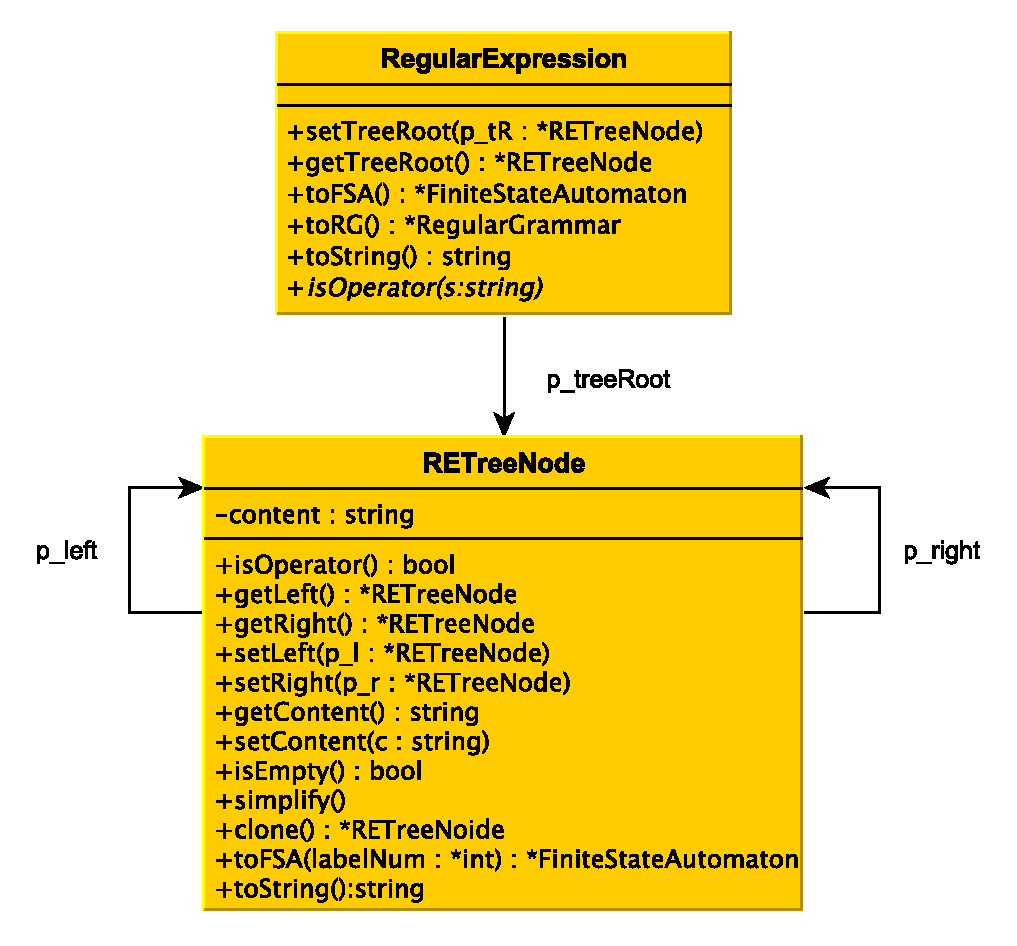
\includegraphics[keepaspectratio]{objectsToInclude/re_uml_ds.pdf}
 \caption{UML Diagramm zu \textit{RegularExpression} und \textit{RETreeNode}}
\label{fig:UMLRegEx}
\end{figure}

\section{Einlesen von Regulären Ausdrücken}
\subsection*{Dateiformat}
Das gewählte Dateiformat ist sehr simpel. Der reguläre Ausdruck wird einfach in einer einzelnen Zeile in einer Textdatei gespeichert. Die Datei sollte nur ASCII-Zeichen enthalten.
\subsection*{Parser}
Das Parsen von Regulären Ausdrücken ist in der Klasse REReaderWriter
implementiert. Während des Parsens wird die Eingabezeichenfolge von links nach
rechts durchgelaufen und der Ausdrucksbaum von unten nach oben aufgebaut.

Somit ähnelt der Prozess dem eines Shift-Reduce-Parsers\cite{RegExShiftReduce}, der
jedoch nicht nach formalen Methoden konstruiert wurde.

\section{Konvertierungen}

\subsection{Konvertierung zu Endlichem Automaten}

Bei der Konvertierung eines Regulären Ausdrucks zu einem endlichen Automaten
wird der Ausdrucksbaum in symmetrischer Reihenfolge (in-order) durchlaufen und für
jeden Knoten ein Automat erstellt. Die Konvertierung wurde im Rahmen des
Projektes selbstständig entworfen. Das Ergebnis der Konvertierung ist ein nichtdeterministischer
endlicher Automat.

\subsubsection{Literal}
Enthält ein Knoten ein Literal, so wird ein Automat
einem Start- und einem Endzustand erzeugt. Der
Startzustand erhält einen Übergang zum Endzustand
mit dem Literal als Eingabe.

\begin{figure}[h]
  \centering
  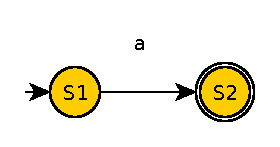
\includegraphics{objectsToInclude/re_fsa_a.pdf}
  \caption{FSA für $a$}
\label{fig:literal}
\end{figure}

\subsubsection{Konkatenation}
Bei einer Konkatenation wird der Automat des
rechten Knotens an den des linken angehängt.
Dazu erhalten alle Endzustände des linken
Automaten einen Übergang mit leerer Eingabe
zu dem Startzustand des rechten Automaten.
Anschließend sind alle Endzustände des linken
Automaten nicht mehr Endzustände und der
Starzustand des rechten Automaten ist kein
Startzustand mehr.

\begin{figure}[h]
  \centering
  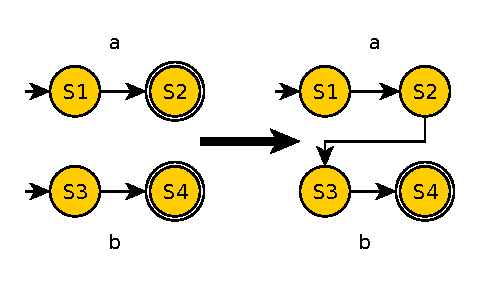
\includegraphics{objectsToInclude/re_fsa_aANDb.pdf}
  \caption{FSA für $a.b$}
\label{fig:Konkatenation}
\end{figure}

\subsubsection{Alternative}
Bei einem Knoten, der eine
Alternative darstellt wird ein neuer
Automaterzeugt, dessen
Startzustand leere Übergänge zu den
Startzuständen der Automaten des
linken und rechten Nachfolgers hat.

\begin{figure}[h]
  \centering
  \includegraphics{objectsToInclude/re_fsa_aOrb.pdf}
  \caption{FSA für $a|b$}
\label{fig:Alternative1}
\end{figure}

\subsubsection{Kleene-Stern}
Enthält ein Knoten einen Kleene-Stern, so wird nur mit dem Automaten des linken
Nachfolgers gearbeitet. Alle Endzustände des Automaten erhalten leere Übergänge
zum Startzustand. Der Startzustand wird auch zu einem Endzustand.

\begin{figure}[h]
  \centering
  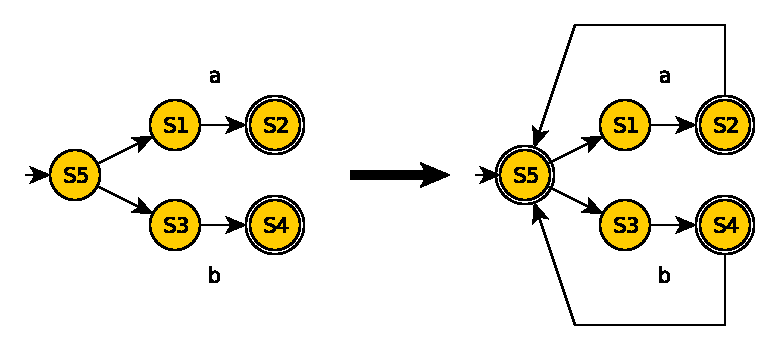
\includegraphics{objectsToInclude/re_fsa_(aOrb)STAR.pdf}
  \caption{FSA für $(a|b)*$}
\label{fig:Kleene-Stern}
\end{figure}

\subsubsection{Entfernung der unnötigen leeren Übergänge}
In vielen Fällen sind die bei der Konvertierung entstandenen Zustände mit leeren
Übergängen unnötig.

Die implementierten Minimierungs-Algorithmen (Moore und Table-Filling) sind
allerdings nicht in der Lage diese unnötigen Zustände und Übergänge zu entfernen.
Daher wurde ein eigener Algorithmus entworfen der möglichst alle Knoten welche mit
leeren Übergängen verbunden sind zu vereinen, solange dies die akzeptierte Sprache
nicht verändert.

In diesem Algorithmus werden alle Zustände des Automaten durchlaufen und für
jeden Zustand seine ausgehenden Kanten.

Wird eine leere Kante auf sich selbst gefunden, so wird diese einfach gelöscht.

Werden leere Transitionen zu anderen Zuständen gefunden so können der
Ausgangszustand und alle Zielzustände unter Umständen zu einem Zustand vereint
werden. Dies kann nur unter der Bedingung geschehen, dass alle Zielzustände keine
weiteren Eingangszustände haben, da sonst beim Vereinen der Zustände die Sprache
verändert würde.

Wird eine nicht-leere, ausgehende Kante gefunden so kann der Zustand nicht einfach
mit anderen Zuständen zu denen er leere Übergänge hat vereint werden, da auch
dann die akzeptierte Sprache verändert werden würde.

Dieser Durchlauf wird so-oft durchgeführt, bis keine Vereinigungen mehr gemacht
werden konnten.

Somit werden die meisten unnötigen Zustände und leeren Übergänge entfernt.


